\documentclass[11pt]{article}
\usepackage[margin=1.2in]{geometry}
\usepackage{graphicx}
% Figures live in ../figures/ in cascadia-curiosities; they sat beside this file
% in the pre-migration submission folder. Both are searched so the source is
% portable to a flat submission bundle without editing the \includegraphics calls.
\graphicspath{{../figures/}{./}}
\usepackage{booktabs}
\usepackage{amsmath}
\usepackage{microtype}
\usepackage[hidelinks]{hyperref}
\usepackage{setspace}
\onehalfspacing

\title{The Combinatorics of Sibling Conflict:\\
\large Why Family Size Creates an Exponential, Not Linear,\\
Increase in Potential Points of Conflict}
\author{Aaron Robbins}
\date{August 2026}

\begin{document}
\maketitle

\noindent
I have four children, each two years apart. I grew up with one sibling, so the
dynamics of a larger family were new to me, and what kept striking me was that the
number of distinct ways my kids could get into a fight seemed never-ending. So I set
out to count it. The answer, for four children, is 25. In general, the number of ways
$n$ children can split into two opposing sides, with the remaining children
uninvolved, is
\[
\frac{3^{n} - 2\cdot 2^{n} + 1}{2},
\]
which is the Stirling number of the second kind $S(n+1,3)$, and it grows
exponentially with family size. Having the number changed how I read the noise in my
own house, and it bears on something parents and researchers alike observe: larger
families report more relational strain than smaller ones, and the strain seems to
grow faster than the family does. The explanation on offer here is combinatorial, not
psychological. Sociologists started counting family structure a long time ago;
Bossard \cite{bossard1945} counted relationships and Kephart \cite{kephart1950}
counted subgroups. What follows extends their arithmetic to opposing-sides conflict
configurations and connects it to the modern literature on coalition structure
generation in cooperative game theory. To be clear at the outset: I make no claim
that this formula predicts how often real siblings fight, or how badly. It measures
the size of the possibility space in which conflict can occur. My suggestion is that
the size of that space, rather than any single behavioral trait, may be an
underappreciated variable in family cohesion research.

\section*{1. The problem as commonly understood}

Sibling relationship research has long documented that coalition formation is a real
and recurring feature of family systems. Siblings form alliances to gain leverage
against parents or against other siblings, and these coalitions shift over time.
Structural family therapy treats the coalition, a joint action of two family members
against a third, as a central unit of analysis \cite{minuchin1974}. Caplow
\cite{caplow1968} showed that triads across social life, families included, tend
naturally to divide into two-against-one formations. Contemporary reviews confirm
that sibling dynamics operate within larger family system dynamics and help
constitute them \cite{mchale2012, bank1982}. All of this literature describes
coalitions qualitatively, as social and emotional phenomena shaped by birth order,
gender, and parenting style.

A quantitative tradition also exists, though it is older and largely dormant. Bossard
\cite{bossard1945} proposed a ``law of family interaction'': with each person added
to a family, the number of dyadic relationships grows as the triangular numbers,
$n(n-1)/2$. Kephart \cite{kephart1950} extended the count to possible subgroupings
and showed that the combinatorial structure of a household grows far faster than its
headcount. Neither tradition asks the question taken up here. The question is not how
many relationships or subgroups a family contains. It is how many distinct ways the
children can divide into opposing sides, and how that number scales.

\section*{2. The combinatorial framework}

Game theorists and multi-agent systems researchers have studied coalition structure
generation extensively. Their central question is how many ways a set of $n$ agents
can be partitioned into cooperating or opposing groups, and how to search that space
efficiently \cite{sandholm1999, rahwan2015}. The framework transfers directly to
sibling groups once each child is treated as an agent who can be on one side of a
conflict, on the opposing side, or uninvolved.

A conflict configuration is then an unordered pair of disjoint, nonempty subsets of
the $n$ children. The two subsets are the sides; any remaining children sit it out.
Each child can be assigned to side $A$, side $B$, or neither, giving $3^{n}$
assignments. Inclusion-exclusion removes the $2\cdot 2^{n} - 1$ assignments in which
a side is empty, and dividing by two accounts for the interchangeable labels $A$ and
$B$:
\begin{equation}
C(n) \;=\; \frac{3^{n} - 2\cdot 2^{n} + 1}{2}.
\label{eq:main}
\end{equation}
Concretely, take three children named A, B, and C. The six configurations are the
three one-on-one disputes (A against B with C uninvolved, and its two counterparts)
and the three two-against-one splits ($\{A,B\}$ against C, and its two counterparts).

The expression in equation~\eqref{eq:main} is not ad hoc. It equals $S(n+1,3)$, a
Stirling number of the second kind, and it appears in the On-Line Encyclopedia of
Integer Sequences as A000392, where one of its listed characterizations is exactly
this: the number of ways to form disjoint unions of two nonempty subsets of an
$n$-element set \cite{oeis}. Table~\ref{tab:values} collects the values for $n = 1$
through $8$ next to Bossard's dyadic count. Figure~\ref{fig:typical} plots the range
where most families actually live, $n \le 4$, with every value readable.
Figure~\ref{fig:growth} extends the range to $n = 8$, where the shape of the growth
takes over.

\begin{table}[htbp]
\centering
\caption{Possible conflict configurations, $C(n)$ of equation~\eqref{eq:main},
against pairwise relationships, $n(n-1)/2$. All values are exact.}
\label{tab:values}
\begin{tabular}{@{}rrr@{}}
\toprule
Children $n$ & Conflict configurations $C(n)$ & Sibling pairs $n(n-1)/2$ \\
\midrule
1 & 0     & 0  \\
2 & 1     & 1  \\
3 & 6     & 3  \\
4 & 25    & 6  \\
5 & 90    & 10 \\
6 & 301   & 15 \\
7 & 966   & 21 \\
8 & 3{,}025 & 28 \\
\bottomrule
\end{tabular}
\end{table}

\begin{figure}[htbp]
\centering
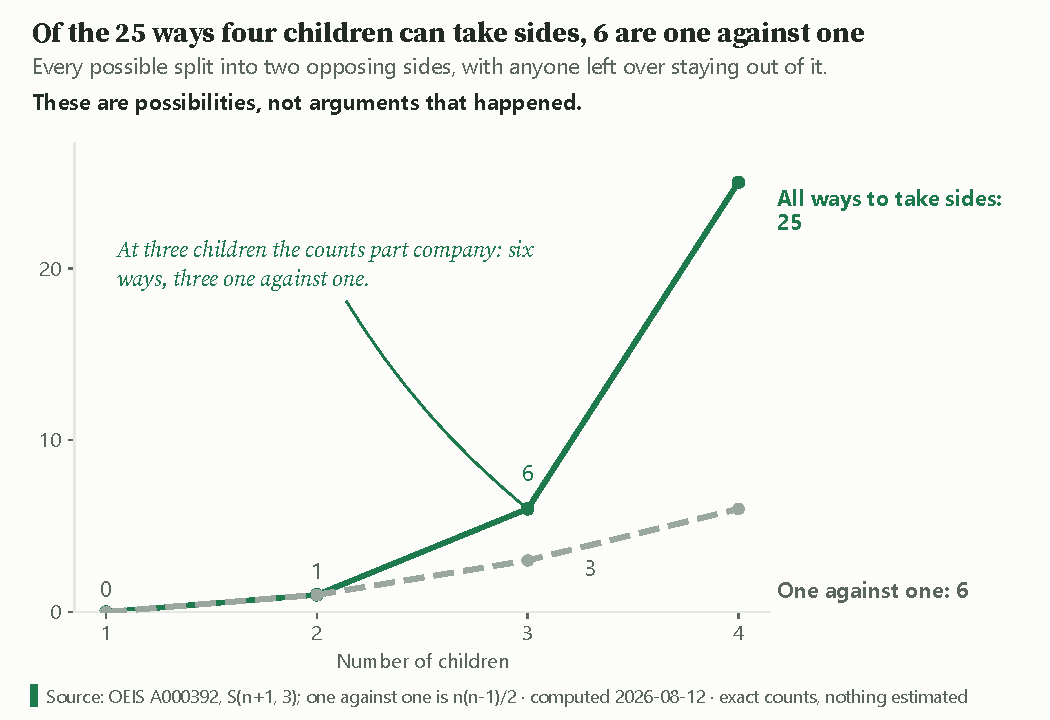
\includegraphics[width=0.95\textwidth]{figureA_design.pdf}
\caption{Conflict configurations $C(n) = (3^{n} - 2\cdot 2^{n} + 1)/2$, the ways $n$
children can split into two opposing sides with the remaining children uninvolved,
against pairwise relationships $n(n-1)/2$, for the family sizes most readers actually
have ($n = 1$ to $4$). The two counts agree at one and two children and diverge from
three onward: 6 configurations against 3 pairs at $n=3$, then 25 against 6 at $n=4$.
The counts are a possibility space, exact by construction. They carry no claim about
the frequency or severity of actual conflicts.}
\label{fig:typical}
\end{figure}

\begin{figure}[htbp]
\centering
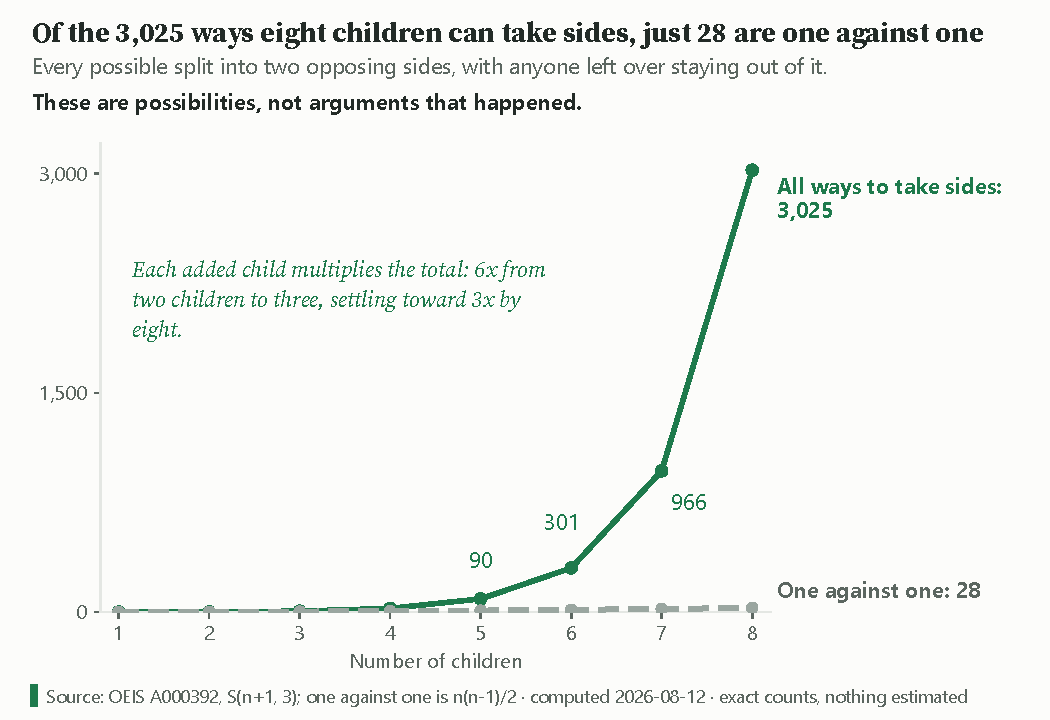
\includegraphics[width=0.95\textwidth]{figure1_design.pdf}
\caption{The same two counts extended to $n = 8$. Successive values of $C(n)$
approach a constant ratio of 3 (90, 301, 966, 3{,}025), so the growth is exponential,
while the dyadic count below it is quadratic and reaches only 28. The values of
Figure~\ref{fig:typical} sit in the flat left edge of this frame. As before, the
counts are a possibility space, not observed conflicts.}
\label{fig:growth}
\end{figure}

The shape of the growth is the point. The jump from two children to three is
six-fold. The jump from three to four multiplies the count by roughly four again.
Nothing linear behaves this way, and no quadratic does either; the growth rate tracks
$3^{n}$. Bossard's dyadic count, by contrast, is quadratic. His framework registers
the difference between two children and eight as 1 relationship versus 28. The
conflict-configuration space registers it as 1 versus 3{,}025.

One note on related formalisms. A similar ally/opponent/neutral trichotomy underlies
``three-way conflict analysis'' in the tradition of Pawlak's conflict models, which
has been applied to labor and political disputes \cite{lang2017}. That literature
analyzes the structure of a given conflict. This article counts the space of
structures available.

\section*{3. Why this matters, and what this article does not claim}

Whether the number of possible conflict configurations determines actual conflict
frequency, severity, or long-term relational outcomes is an empirical question, and
nothing here settles it. Many families with high theoretical conflict potential
remain close. Some two-child families fracture. What the framework offers is a way to
quantify the possibility space that parents, therapists, and researchers are
implicitly reacting to when they describe larger families as harder to manage or more
prone to shifting alliances.

The empirical literature gives the reframing some initial traction. Sibling
estrangement in adulthood is common enough to measure at scale; in German panel data,
28\% of respondents reported at least one episode of estrangement from a sibling
\cite{hank2023}. Recent work on medium-to-large families finds that sibling
relationship quality in larger sibships is multifaceted, with substantial variation
across dyads within the same family \cite{jensen2026}. Within-family variation across
dyads is what a large configuration space would predict, though it is consistent with
other explanations too. The concrete proposal for family cohesion research is this:
test whether reported conflict frequency, coalition instability, or estrangement
outcomes correlate with the theoretical conflict space of a family, independent of
family size alone.

\section*{4. Directions for further research}

Researchers with access to sibling relationship data could test whether the
theoretical conflict space correlates with reported measures of sibling closeness,
conflict frequency, or estrangement in adulthood. Another open question is whether
particular family structures matter: evenly split coalitions are available to
four-child families, for example, while three-child families are limited to
one-against-one and two-against-one forms, and those structural differences might
correlate with different relational outcomes. The framework could also be extended to
model coalition stability over time, since sibling alliances are known to shift, and
the count developed here is static; it says which configurations are possible, not
which ones occur or persist. The coalition structure generation literature has built
tools for reasoning about exactly such spaces \cite{rahwan2015} and may supply the
machinery for that extension.

\section*{Conclusion}

The number of possible sibling conflict configurations grows exponentially with
family size, not linearly. Why some large families remain close while others fracture
is a question this article leaves alone. What it offers is a map of the terrain: a
measure of how much structural complexity a family navigates as it grows. Bossard and
Kephart began the mapping three-quarters of a century ago with relationships and
subgroups. Extending it to opposing-sides configurations reveals a possibility space
vastly larger still. I offer the framework in the hope that it proves useful to
parents seeking context for what they are experiencing, and to researchers who want
to test whether this structural complexity is itself a meaningful variable in family
cohesion outcomes.

\begin{thebibliography}{12}

\bibitem{bank1982}
S.~P. Bank and M.~D. Kahn, \emph{The Sibling Bond}, Basic Books, New York, 1982.

\bibitem{bossard1945}
J.~H.~S. Bossard, The law of family interaction, \emph{American Journal of
Sociology} \textbf{50} (1945), no.~4, 292--294.

\bibitem{caplow1968}
T.~Caplow, \emph{Two Against One: Coalitions in Triads}, Prentice-Hall, Englewood
Cliffs, NJ, 1968.

\bibitem{hank2023}
K.~Hank and A.~Steinbach, Sibling estrangement in adulthood, \emph{Journal of Social
and Personal Relationships} \textbf{40} (2023), no.~4, 1277--1287.

\bibitem{jensen2026}
A.~C. Jensen, S.~Ashby, N.~M. Noorda, and J.~Jasperson, The more, the merrier? Young
adults' sibling relationship quality in medium to large families, \emph{Journal of
Social and Personal Relationships} (2026), doi:10.1177/02654075241302240.

\bibitem{kephart1950}
W.~M. Kephart, A quantitative analysis of intragroup relationships, \emph{American
Journal of Sociology} \textbf{55} (1950), no.~6, 544--549.

\bibitem{lang2017}
G.~Lang, D.~Miao, and M.~Cai, Three-way decision approaches to conflict analysis
using decision-theoretic rough set theory, \emph{Information Sciences}
\textbf{406--407} (2017), 185--207.

\bibitem{mchale2012}
S.~M. McHale, K.~A. Updegraff, and S.~D. Whiteman, Sibling relationships and
influences in childhood and adolescence, \emph{Journal of Marriage and Family}
\textbf{74} (2012), no.~5, 913--930.

\bibitem{minuchin1974}
S.~Minuchin, \emph{Families and Family Therapy}, Harvard University Press, Cambridge,
MA, 1974.

\bibitem{oeis}
OEIS Foundation Inc., Sequence A000392: Stirling numbers of second kind $S(n,3)$,
\emph{The On-Line Encyclopedia of Integer Sequences}, \url{https://oeis.org/A000392}.

\bibitem{rahwan2015}
T.~Rahwan, T.~P. Michalak, M.~Wooldridge, and N.~R. Jennings, Coalition structure
generation: A survey, \emph{Artificial Intelligence} \textbf{229} (2015), 139--174.

\bibitem{sandholm1999}
T.~Sandholm, K.~Larson, M.~Andersson, O.~Shehory, and F.~Tohm\'e, Coalition structure
generation with worst case guarantees, \emph{Artificial Intelligence} \textbf{111}
(1999), no.~1--2, 209--238.

\end{thebibliography}

\bigskip
\noindent\rule{0.3\textwidth}{0.4pt}

\medskip
\noindent
\textsc{Aaron Robbins} \\
Robbins Analytics \\
\texttt{ajayrobbins@hotmail.com}

\end{document}
